%%%%%%%%%%%%%%%%%%%%%%%%%%%%%%%%%%%%%%%
\thesisspacing % CHAPTER
% COPY THEM IN ANY NEW CHAPTER
%%%%%%%%%%%%%%%%%%%%%%%%%%%%%%%%%%%%%%%

This section presents the results of the CNN models developed for financial market prediction and their subsequent evaluation through backtesting. Two models are highlighted: one with poor training performance and another with better training outcomes. The results include both the model training phases and their respective backtesting performances using QSTrader.

\section{Model Training Results}

\subsection{Poorly Performing CNN Model}

The first CNN model displayed suboptimal performance during the training phase. As shown in Figure~\ref{fig:poor_model_training}, this model struggled to accurately identify market trends and predominantly generated short signals, failing to capture upward market movements. This resulted in an inability to effectively predict bullish conditions.

\begin{figure}[h!]
    \centering
    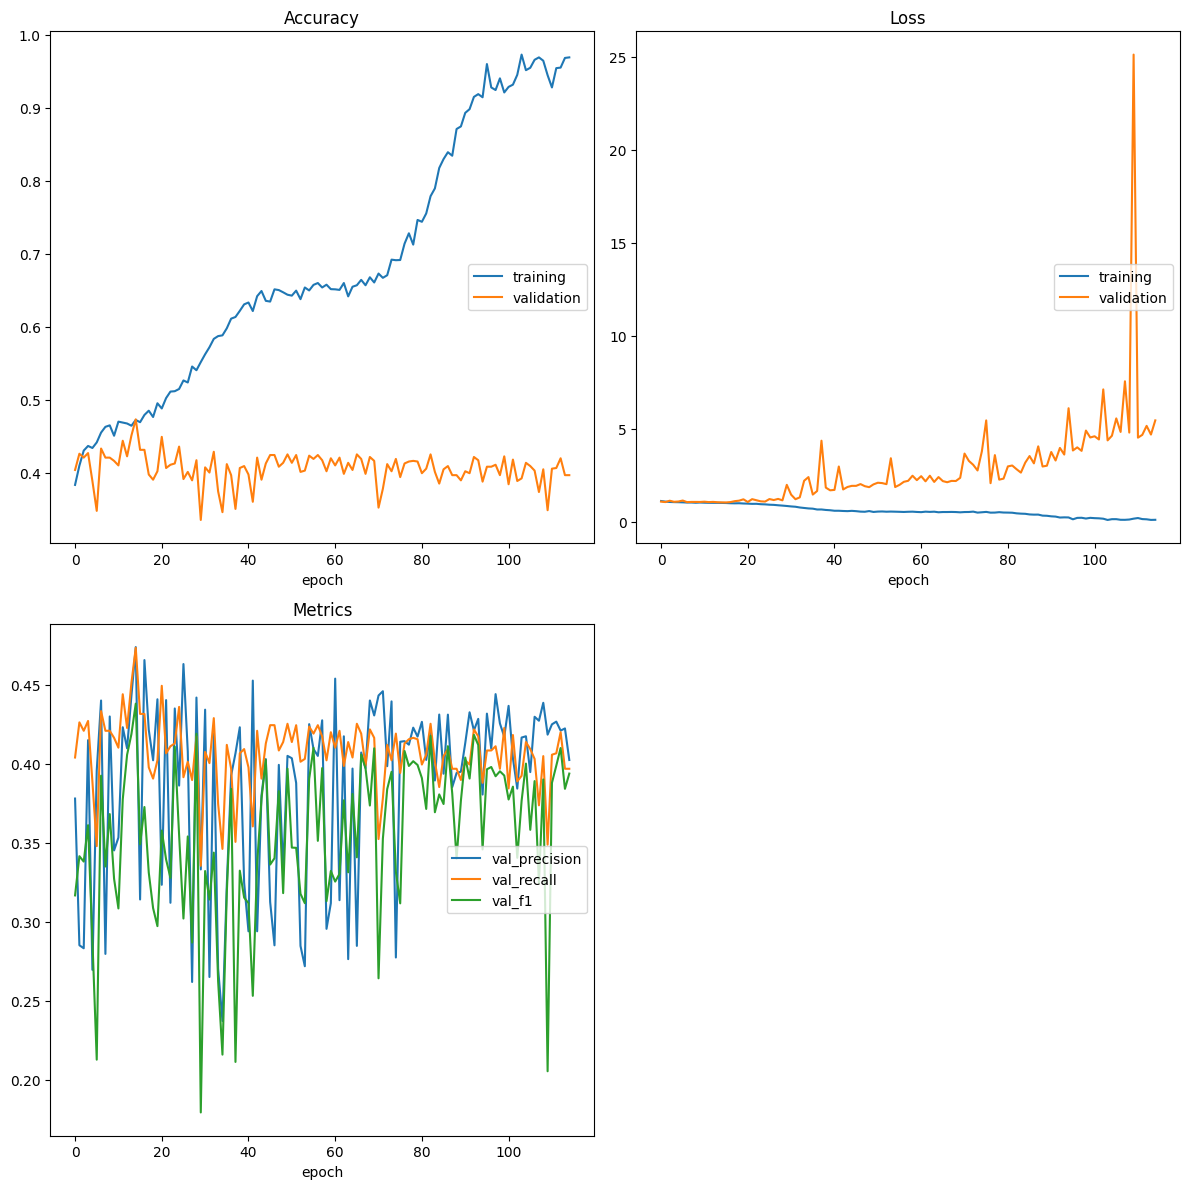
\includegraphics[width=0.7\textwidth]{chapters/Chap3/CNN_Fail_Training.png}
    \caption{Training performance of the poorly performing CNN model, predominantly generating short signals.}
    \label{fig:poor_model_training}
\end{figure}

\subsection{Well-Performing CNN Model}

In contrast, the second CNN model demonstrated significantly better training performance. As depicted in Figure~\ref{fig:good_model_training}, this model was able to effectively learn from the training data, identifying both long and short signals with greater accuracy. The balanced signal generation indicates a more refined model capable of capturing a range of market conditions.

\begin{figure}[h!]
    \centering
    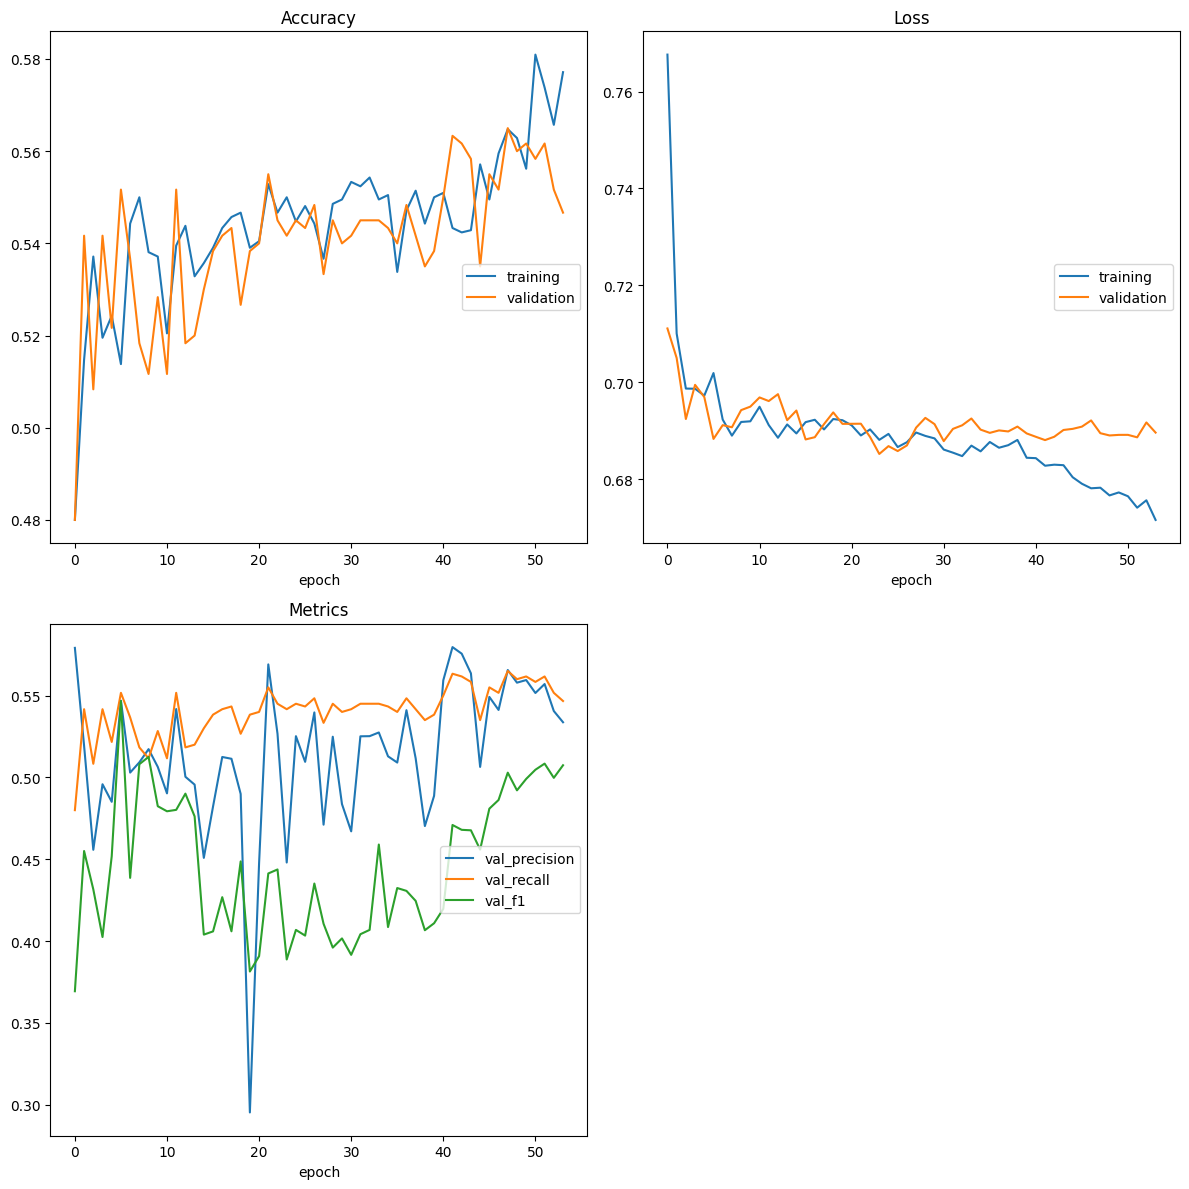
\includegraphics[width=0.7\textwidth]{chapters/Chap3/CNN_Working_Training.png}
    \caption{Training performance of the well-performing CNN model, showing a balanced understanding of both long and short signals.}
    \label{fig:good_model_training}
\end{figure}

\section{Backtesting Results}

\subsection{Backtest of Poorly Performing CNN Model}

The backtest results for the poorly performing model, as shown in Figure~\ref{fig:failed_backtest}, reflect its training deficiencies. The model’s inability to accurately generate long signals resulted in a predominantly short-biased strategy, which underperformed during bullish market conditions. The backtest metrics indicate a low Sharpe ratio, high maximum drawdown, and negative CAGR, highlighting the model's poor risk-adjusted performance.

\begin{figure}[h!]
    \centering
    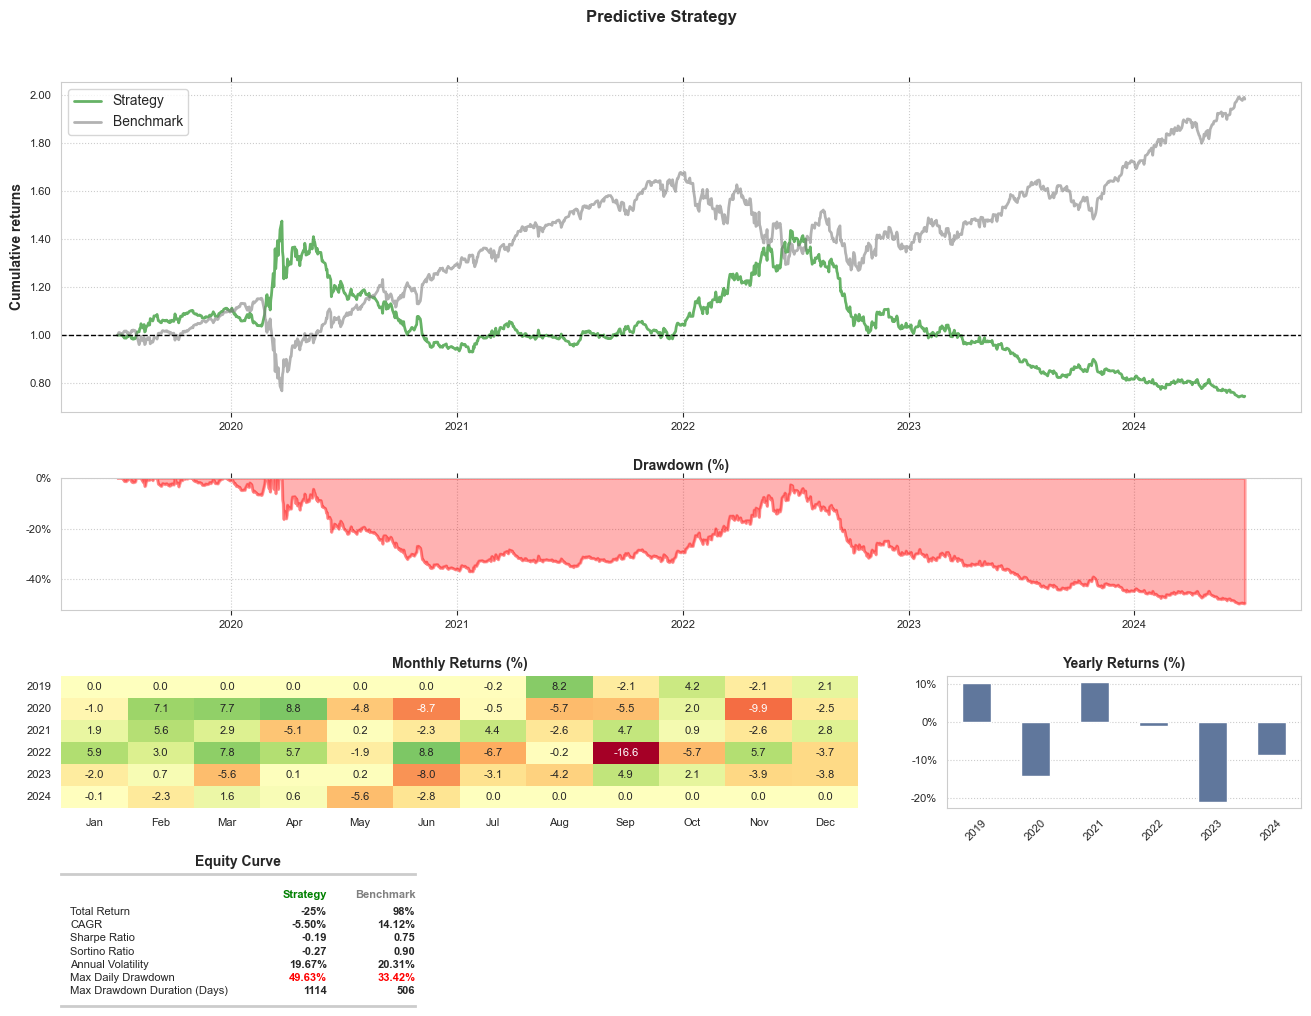
\includegraphics[width=0.7\textwidth]{chapters/Chap3/Model_Fail_Backtest.png}
    \caption{Backtest results for the poorly performing CNN model, showing a failure to generate effective long signals.}
    \label{fig:failed_backtest}
\end{figure}

\subsection{Backtest of Well-Performing CNN Model}

Figure~\ref{fig:successful_backtest} presents the backtest results for the well-performing CNN model. This model effectively generated both long and short signals, resulting in a more balanced and adaptive trading strategy. The backtest metrics demonstrate a higher Sharpe ratio, lower drawdown, positive CAGR, and reduced volatility, indicating superior risk management and return optimization compared to the poorly performing model.

\begin{figure}[h!]
    \centering
    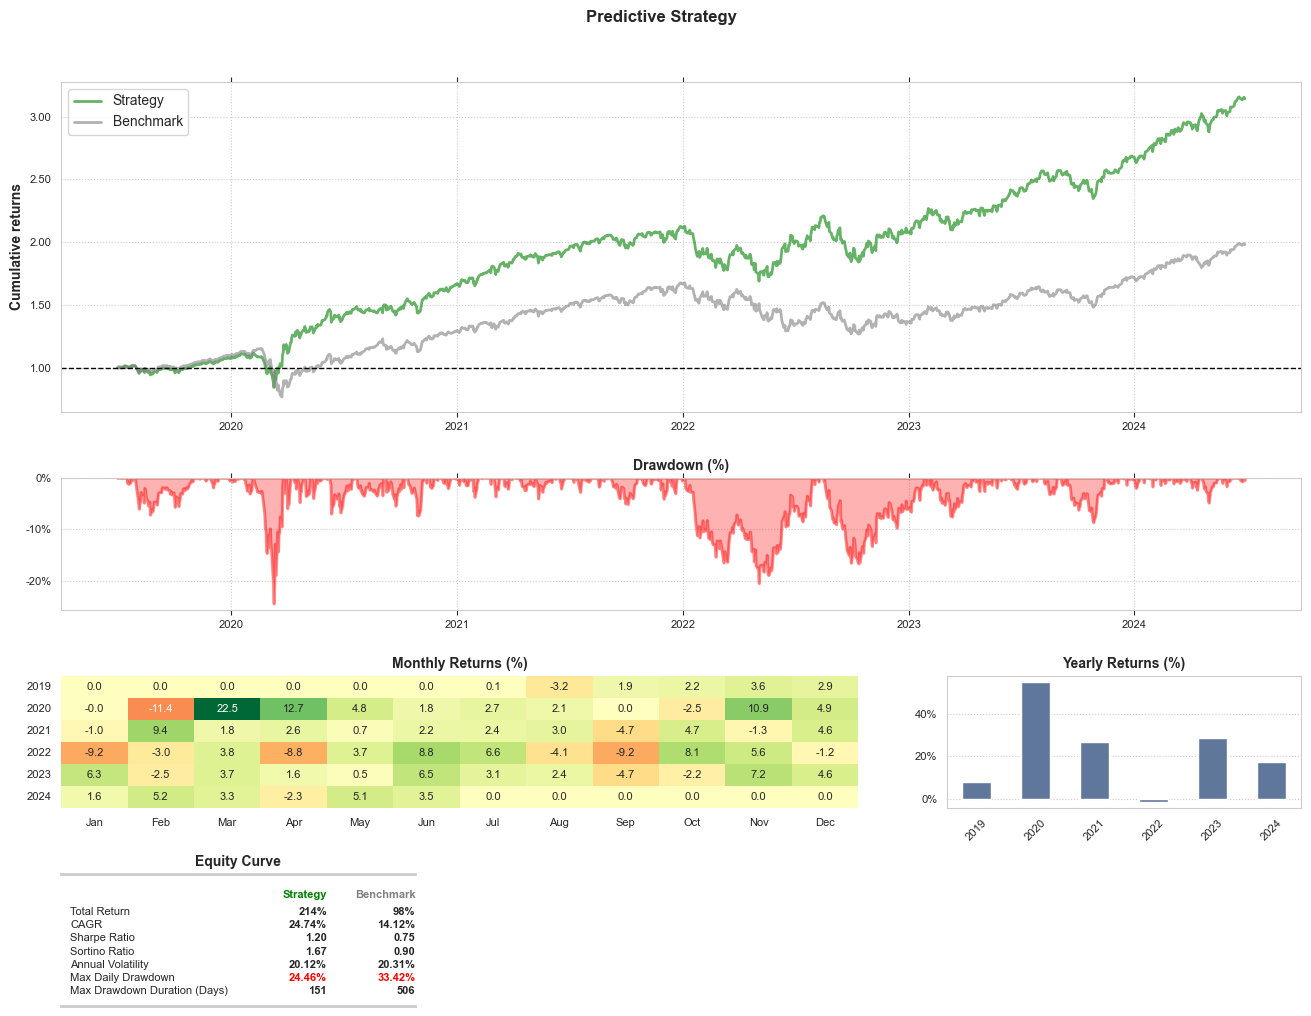
\includegraphics[width=0.7\textwidth]{chapters/Chap3/Model_Working_Backtest.png}
    \caption{Backtest results for the well-performing CNN model, demonstrating effective signal generation and improved portfolio performance.}
    \label{fig:successful_backtest}
\end{figure}

\section{Performance Analysis}

Table~\ref{tab:performance_metrics} summarizes the key performance metrics for both models based on their backtesting results. These metrics, including drawdown, Sharpe ratio, CAGR, and volatility, provide a comparative analysis of the two models’ effectiveness in predicting market movements and managing risk.

\begin{table}[h!]
    \centering
    \caption{Performance Metrics for Trained CNN Models}
    \label{tab:performance_metrics}
    \begin{tabular}{lcc}
        \toprule
        \textbf{Metric} & \textbf{Poorly Performing Model} & \textbf{Well-Performing Model} \\
        \midrule
        Drawdown (\%) & 49.63 & 24.46 \\
        Sharpe Ratio & 0.19 & 1.20 \\
        CAGR (\%) & -5.50 & 24.74 \\
        Volatility (\%) & 19.67 & 20.12 \\
        \bottomrule
    \end{tabular}
\end{table}
